\section{Erweiterung der Filterkombinationen}
\thispagestyle{fancy}

Im Zuge dieser Arbeit wurden für eine Erhöhung der Messpunkte und Verringerung von Rauschen bei der leistungsdichteabhängigen Messung der IQE die Anzahl der Filterkombination erhöht. Dafür wurden die alten zwei Filterräder durch drei neue ersetzt. 
%
\begin{figure}[ht!]
    \centering
    \begin{minipage}[t]{1\linewidth}
        \centering
        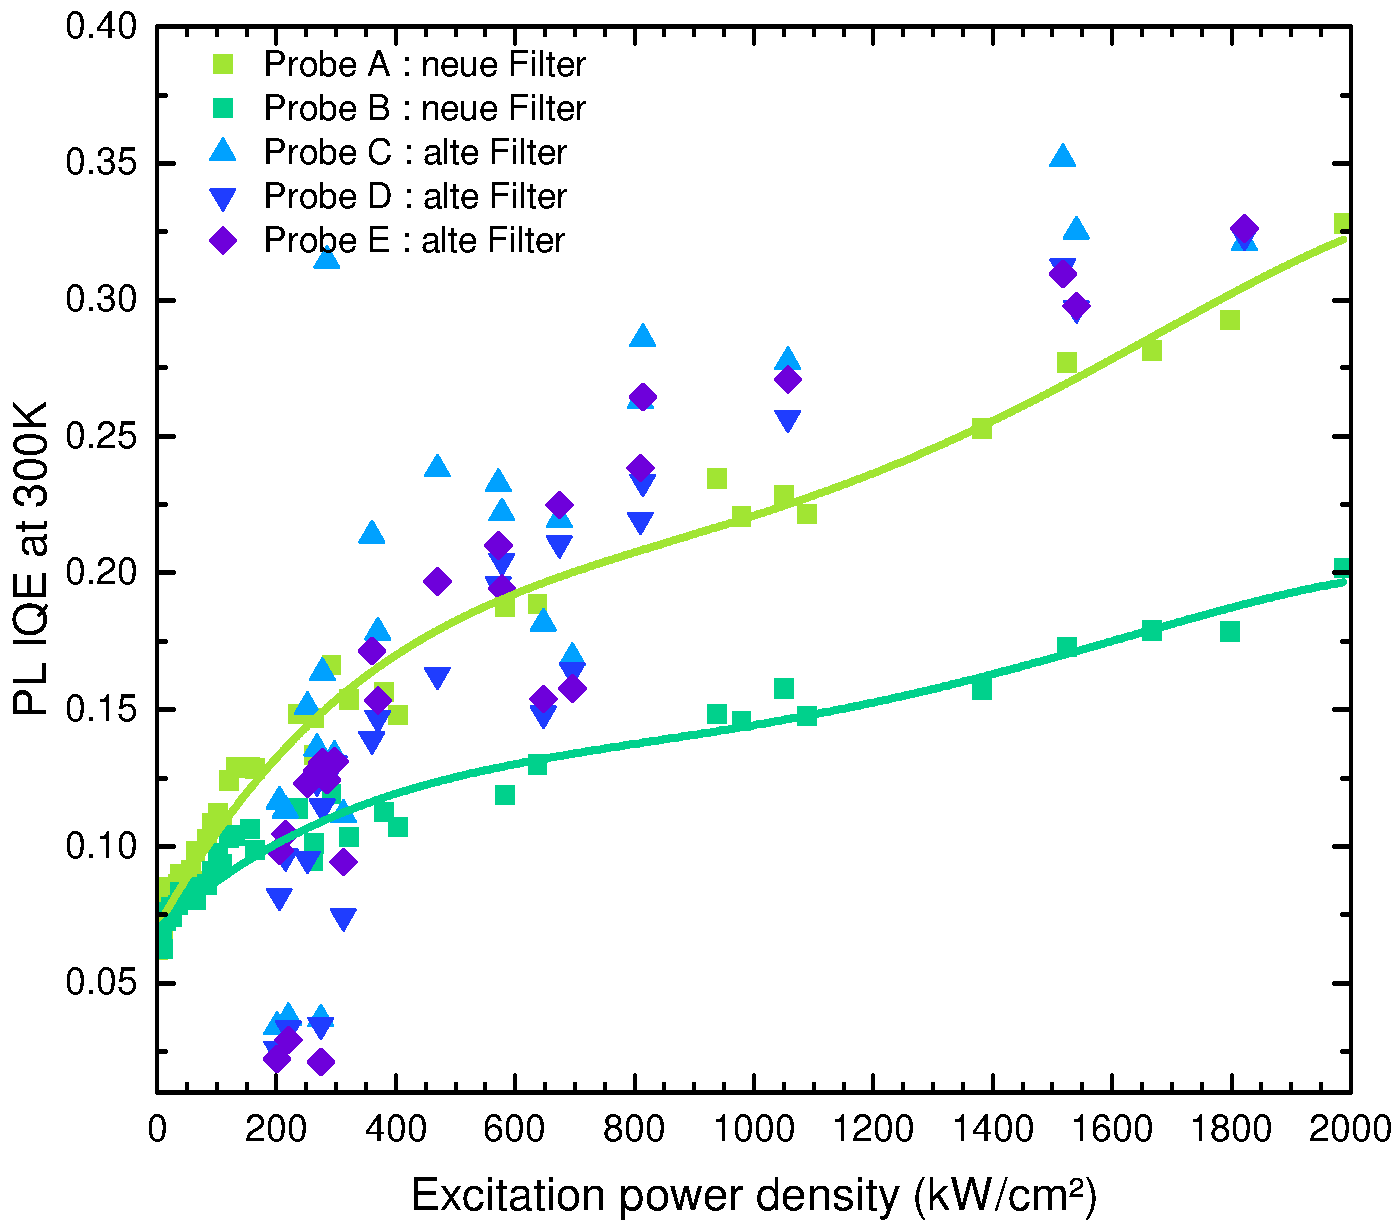
\includegraphics[width = 0.49\linewidth]{Bilder/AuswertungNovemeberKorr1VergleichFilter.pdf}
        \caption{Vergleich der Messung von insgesamt 5 ähnlichen Proben. 3 Proben (blau) wurden mit dem alten Setup gemessen. 2 Proben (grün, durchgezogene Linie) wurden mit dem neuen Setup gemessen. %Die Präzision in tieferen Anregungsleistungsdichtenbereichen ist für das neue Setup deutlich %erhöht. Das Rauschen fällt ebenfalls deutlich geringer aus. 
        }
        \label{fig:vergleichFilter}
    \end{minipage}
\end{figure}
%
\newpage
Durch die erhöhte Anzahl möglicher Filterkombinationen ist es möglich, statt nur 27 verschiedene Messpunkte 61 zu messen. Es ist deutlich sichtbar, dass speziell der Bereich der geringen Anregungsleistungsdichten viel besser aufgelöst werden kann (Abb: [\ref{fig:vergleichFilter}]). Und wie zu erwarten, sinkt die Intensität nicht mehr plötzlich ab einer Anregungsleistungsdichte von $200 \frac{kW}{cm^2}$ auf 0, sondern weist stattdessen eine Ordinate größer Null auf. Wie laut Gleichung \ref{eq:dopediqe} zu erwarten wäre. Somit hat die Erweiterung und Verbesserung der Filterräder, nicht nur mehr Präzision und weniger Rauschen als Ergebnis, sondern liefert nun auch physikalisch verwertbarere Werte.
%
